\documentclass[10pt,a4paper]{article}

\usepackage[a4paper,top=1.7cm,bottom=1.7cm,left=2.2cm,right=2.2cm,footskip=0.9cm]{geometry}
\usepackage{fontspec}
\usepackage{xeCJK}
\usepackage{graphicx}
\usepackage{booktabs}
\usepackage{tabularx}
\usepackage{array}
\usepackage[table]{xcolor}
\usepackage{titlesec}
\usepackage{enumitem}
\usepackage{caption}
\usepackage{float}
\usepackage[hidelinks]{hyperref}

% Fonts: PingFang TC for CJK, SF Pro for Latin
\setmainfont{SF Pro Text}[BoldFont={* Semibold}, ItalicFont={* Regular Italic}, BoldItalicFont={* Semibold Italic}]
\setsansfont{SF Pro Display}[BoldFont={* Semibold}]
\setCJKmainfont{PingFang.ttc}[Path=/jupyter/fonts/中文/, FontIndex=2, BoldFont=PingFang.ttc, BoldFeatures={FontIndex=10}]
\setCJKsansfont{PingFang.ttc}[Path=/jupyter/fonts/中文/, FontIndex=2, BoldFont=PingFang.ttc, BoldFeatures={FontIndex=10}]
\xeCJKsetup{CJKecglue={\hskip 0.25em plus 0.08em minus 0.04em}}
\xeCJKDeclareCharClass{Default}{"2013, "2212, "2192, "00D7}

% Spacing: 10.5pt on 17.5pt leading for body text
\renewcommand{\normalsize}{\fontsize{10.5pt}{17.5pt}\selectfont}
\renewcommand{\small}{\fontsize{9.5pt}{15pt}\selectfont}
\renewcommand{\footnotesize}{\fontsize{8.5pt}{13pt}\selectfont}
\setlength{\parindent}{0pt}
\setlength{\parskip}{5pt}

\definecolor{accent}{HTML}{2A78D6}
\definecolor{ink}{HTML}{1D1D1F}
\definecolor{muted}{HTML}{6E6E73}
\definecolor{rule}{HTML}{D2D2D7}
\definecolor{todo}{HTML}{D03B3B}

\setlist{nosep,leftmargin=1.1em,topsep=3pt,itemsep=2pt}
\setlist[itemize]{label=\textcolor{accent}{\raisebox{0.1ex}{$\bullet$}}}
\usepackage{fancyhdr}
\usepackage{lastpage}
\fancyhf{}
\renewcommand{\headrulewidth}{0pt}
\cfoot{\footnotesize\color{muted}\thepage\ / \pageref*{LastPage}}
\pagestyle{fancy}

\titleformat{\section}{\sffamily\bfseries\fontsize{13pt}{18pt}\selectfont}{\textcolor{accent}{\thesection}}{0.6em}{}
\titlespacing*{\section}{0pt}{12pt}{4pt}

\captionsetup{font={footnotesize,color=muted},labelfont={bf,color=ink},labelsep=quad,skip=5pt}
\captionsetup[table]{name=表,position=top}
\captionsetup[figure]{name=圖}
\arrayrulecolor{rule}
\renewcommand{\arraystretch}{1.15}

% ---- numbers that are still pending render in red; fill them when the runs finish ----
\newcommand{\tbd}{\textcolor{todo}{待補}}
\newcommand{\kaggle}{65.8}        % Kaggle public of the final notebook's CSV: 0.65835 (submission 57807731, 2026-10-30 14:11 UTC, result/minisam-final.csv = output.csv); val with the same chain 0.6535; the old 003+008 ensemble scored 0.63990
\newcommand{\bestval}{63.3}       % best val mIoU (per-image mean, hflip TTA) of the submitted model: final notebook run, EMA weights of epoch 146 (0.6282 without TTA, raw best 0.6270 at epoch 140); the chain cell's 448+hflip value is 0.6337 (bf16 noise)
\newcommand{\bestrun}{最終 run}   % the submitted model: 011's config at 150 epochs, trained inside HW4_315834011.ipynb on a Colab RTX PRO 6000
\newcommand{\unetval}{52.0}       % U-Net best val mIoU in the submitted notebook (epoch 18 of 20, same Colab GPU); the earlier local 3090 Ti run gave 52.2
\newcommand{\unetkaggle}{–}       % U-Net Kaggle public score: not submitted (user holds all submissions as of 2026-10-29 23:35); fill if the user decides to submit output.csv
\newcommand{\bestparams}{42.7M}   % parameter count of the submitted model
\newcommand{\finalval}{65.4}      % val mIoU of the submitted pipeline printed by the notebook: final run, sizes 512/576/640/704/768, hflip, min-area 50 (without min-area 65.0; 011 gave 64.5 / 64.0)
\newcommand{\besttime}{7.3 h}     % wall-clock training time of the submitted model: the mini-SAM cell printed elapsed 435.8 min (06:40-13:55 UTC on the Colab RTX PRO 6000; per-epoch sum 425 min, 2.8 min/epoch; 011 took 289 min for 100 epochs)

\newcommand{\keynum}[2]{%
  \begin{tabular}[t]{@{}c@{}}
    {\sffamily\bfseries\fontsize{17pt}{20pt}\selectfont #1}\\[1pt]
    {\footnotesize\color{muted}#2}
  \end{tabular}}

\begin{document}
\color{ink}

{\sffamily\bfseries\fontsize{18pt}{24pt}\selectfont DL Lab 4　CIHP 人體解析語意分割}\hfill
{\color{muted}黃毓峰　315834011}

\vspace{6pt}
{\renewcommand{\arraystretch}{1}%
\begin{tabularx}{\linewidth}{@{}*{4}{>{\centering\arraybackslash}X}@{}}
\arrayrulecolor{ink}\toprule[0.8pt]\addlinespace[6pt]
\keynum{\unetval}{U-Net val mIoU} &
\keynum{\finalval}{上傳設定 val mIoU，第 6 節} &
\keynum{\kaggle}{Kaggle public} &
\keynum{\bestparams}{\bestrun{} 參數量，訓練 \besttime} \\
\addlinespace[4pt]\arrayrulecolor{rule}\bottomrule
\end{tabularx}}

\section{任務與資料}
CIHP 多人影像的 20 類語意分割，影像與 mask 都是 320×320，mask 值 255 是等比例縮放後的補邊，不參與 loss 與評分。
訓練 28,280 張、驗證 1,000 張、測試 3,961 張。評分是每張影像先對出現的類別算 IoU 取平均，再對所有影像平均。

資料有三個特性決定了後面的設計。
第一，類別極不平衡：背景占有效像素 59.7\%，太陽眼鏡 0.04\%、手套 0.06\%、襪子 0.12\%，左右鞋各 0.21\%。
評分逐張對類別平均，一張圖裡的小物件和大面積的上衣權重相同，漏掉一個小類就掉一大塊分數。
第二，補邊占全部 mask 像素 28.6\%，單張有效比例最低只有 0.28，寬幅影像裡的人很小，尺度差距大。
第三，訓練集內有 137 對完全相同的影像但標註不同，多數只差邊界，是少量標註雜訊；驗證與測試集和訓練集沒有重複，驗證分數可信。

\section{方法}

\begin{minipage}[t]{0.52\linewidth}
\raggedright\setlength{\parskip}{5pt}
\textbf{U-Net 基準}　依作業要求自行實作原始 U-Net：4 層下採樣，通道 64 到 1024，DoubleConv 為 Conv 3×3 → BN → ReLU 兩次，上採樣用 transposed convolution 後與 skip 串接，共 31.0M 參數。

\textbf{Mini-SAM}　最終模型借用 SAM 的結構但全部從零訓練。
編碼器是 Hiera 式的四階段階層 transformer（stride 4/8/16/32）：卷積 stem 到 stride 4，前兩階段用 8×8 視窗注意力，後兩階段全域注意力（448 輸入時只有 784 與 196 個 token）；每個 block 先過 depthwise 3×3 卷積當位置編碼，再過 LayerScale 與 stochastic depth 的注意力與 MLP。
FPN neck 把四個尺度對齊到 256 通道。
解碼器是 SAM 的 two-way transformer：20 個可學習的類別 token 與 stride-16 影像 token 互相做 cross-attention 兩輪，token 經 hypernetwork MLP 產生 mask embedding，與上採樣到 stride 4 的像素 embedding 做內積得到 20 張 mask，再放大回輸入大小。
上採樣路徑如 SAM 2 一樣加入 FPN 的 stride-8 與 stride-4 特徵。
訓練時另外在 stride-4 特徵上接一個逐像素輔助 head 做深度監督。
\end{minipage}\hfill
\begin{minipage}[t]{0.44\linewidth}
\vspace{-6pt}
\captionof{table}{最佳模型的訓練設定（\bestrun）}
\small
\begin{tabularx}{\linewidth}{@{}>{\color{muted}}l >{\raggedright\arraybackslash}X@{}}
\toprule
輸入 & 448×448（影像與 mask 放大 1.4 倍），logits 縮回 320 計分 \\
編碼器 & stem 48，寬度 96/192/384/768，深度 2/2/12/2，head 維度 32，共 \bestparams（320 輸入時 42.6M） \\
Loss & 0.5 CE + 0.5 Dice，輔助 head CE × 0.4，255 不計 \\
Optimizer & AdamW，weight decay 0.05，batch 16 \\
Learning rate & 6×10\textsuperscript{−4}，warmup 5 epoch 後 cosine 到 10\textsuperscript{−5} \\
Epochs & 150（\besttime） \\
正則化 & Drop path 0.2，LayerScale 初值 0.1，梯度裁剪 1.0 \\
權重平均 & EMA 0.9995，每個 epoch 與原始權重各驗證一次，取高者 \\
Augmentation & 仿射縮放 0.5–2.0、平移 ±20\%、旋轉 ±10°（補邊 255）；亮度對比色相；翻轉時交換左右標籤 \\
推論 & bf16，翻轉 TTA（交換左右通道），五尺度 512–768，抑制小於 50 像素的類別（第 6 節） \\
\bottomrule
\end{tabularx}
\end{minipage}

\section{實驗設計}
模型選擇以驗證集的逐張 mIoU 為準（U-Net 也是），不用 val loss，因為兩者在類別不平衡時常常不同步。
U-Net 用模板的 seed 42；mini-SAM 各 run 固定 seed 2026，先以獨立腳本在 Colab 的 RTX PRO 6000 上篩選設定，最終設定再於繳交的 notebook 內從頭訓練一次。

\begin{table}[H]
\centering\small
\caption{各 run 的最佳 val mIoU（\%）}
\label{tab:runs}
\begin{tabularx}{\linewidth}{@{}l >{\raggedright\arraybackslash}X r r@{}}
\toprule
編號 & 設定 & val mIoU & Kaggle public \\
\midrule
U-Net & 原始 U-Net，batch 16，AdamW 10\textsuperscript{−3} OneCycle，20 epoch & \unetval & \unetkaggle \\
002 & mini-SAM 17.1M，batch 16，lr 8×10\textsuperscript{−4}，100 epoch & 57.5（TTA 58.1） & 58.3 \\
003 & 加寬加深版 35.5M（寬度 1.5 倍、第三階段 8 層），100 epoch & 58.8（TTA 59.6） & – \\
004 & 同 002 加 stride-2 mask head、邊緣分支、逐張 Dice & 55.6（TTA 56.9） & – \\
005 & 同 002，前兩階段改用 ConvNeXt 區塊取代視窗注意力 & 57.4（TTA 58.1） & – \\
008 & 003 的第三階段從 8 層加深到 12 層（42.6M） & 59.3（TTA 59.9） & – \\
009 & 003 的 cosine 排程拉長到 150 epoch & 59.9（TTA 60.6） & – \\
014 & 008 的 Dice 換成逐張 Lovász-softmax（直接最佳化逐張 mIoU） & 57.2（TTA 58.3） & – \\
011 & 008 改以 448×448 訓練，logits 縮回 320 計分 & 61.5（TTA 62.1） & – \\
最終 & 011 的排程拉長到 150 epoch，在繳交的 notebook 內訓練（表 1） & 62.8（TTA \bestval） & \kaggle \\
\bottomrule
\end{tabularx}
\end{table}

\section{結果}
圖 \ref{fig:curves} 是各 run 的驗證曲線，表 \ref{tab:runs} 是最佳值。

\begin{figure}[H]
\centering
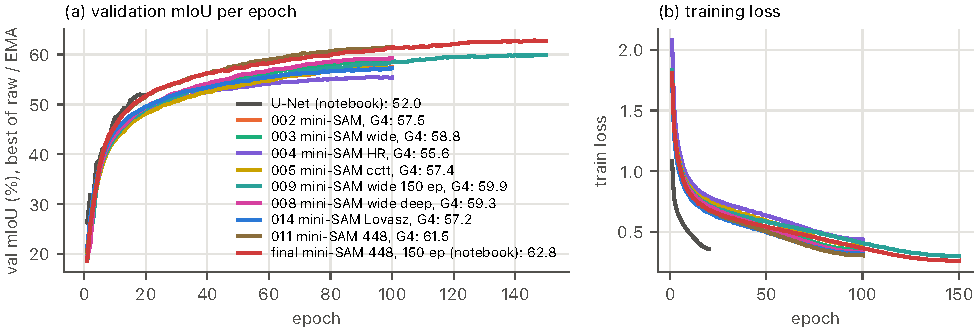
\includegraphics[width=\linewidth]{figures/curves.pdf}
\caption{(a) 每個 epoch 的 val mIoU，取原始與 EMA 權重較高者。(b) 訓練 loss。}
\label{fig:curves}
\end{figure}

\begin{itemize}
  \item \textbf{從零訓練的 mini-SAM 勝過 U-Net 5 到 11 點，最小的 002 只用一半的參數}：U-Net（31.0M）在第 18 epoch 到 \unetval{} 後持平，002（17.1M）到第 100 epoch 仍在緩升，收在 57.5。
  \item \textbf{容量與訓練長度有用，換區塊或 loss 沒用}：003 加寬 1.5 倍、第三階段加深到 8 層得 58.8，008 再加深到 12 層得 59.3；009 只把 003 的排程拉長到 150 epoch 就得 59.9；005 前兩階段換 ConvNeXt 得 57.4（同 002），014 把 008 的 Dice 換成逐張 Lovász 反而得 57.2。
  \item \textbf{輸入解析度是最大的單一增益}：011 把 008 的訓練與推論輸入放大到 448 得 61.5，比 008 高 2.2 點，每個 epoch 慢 1.8 倍；最終 run 同設定跑 150 epoch 得 62.8。
  \item \textbf{EMA 只在前期有用，翻轉 TTA 穩定加 0.6 到 0.8 點}：第 20 epoch 時 EMA 48.2、原始權重 44.7，第 100 epoch 只差 0.2；002 TTA 後 val 58.1、public 58.3，兩者一致，之後只以 val 選模型。
\end{itemize}

\newpage
\section{逐類別分析}

\begin{figure}[H]
\centering
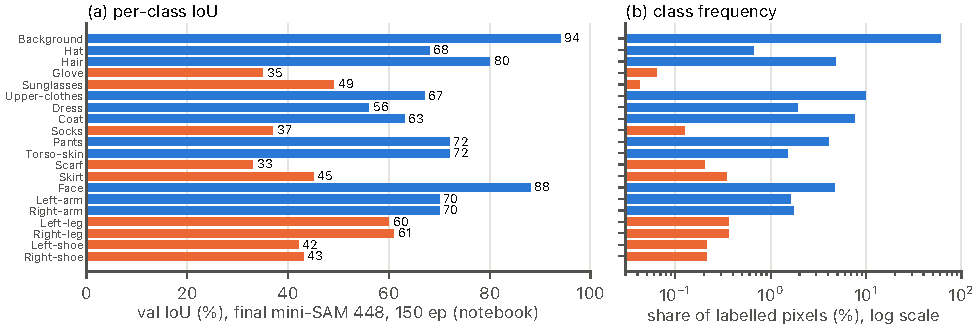
\includegraphics[width=\linewidth]{figures/per_class.pdf}
\caption{(a) 最佳模型在驗證集的逐類別 IoU。(b) 各類別占有效像素的比例，對數刻度；橘色是占比低於 0.5\% 的稀有類。}
\label{fig:cls}
\end{figure}

\begin{itemize}
  \item \textbf{弱項幾乎都是稀有小物件}：手套 35、圍巾 33、襪子 37、鞋 42 與 43，占比都不到 0.22\%。裙子 45 占比 0.34\%，低分主因是和洋裝、褲子外觀重疊，各 run 在 30 到 45 之間跳動。太陽眼鏡只占 0.04\% 卻有 49，難在和鄰近類別相似。
  \item \textbf{左右對稱類別的 IoU 幾乎相同}（手臂 70 與 70、腿 60 與 61、鞋 42 與 43），交換左右標籤的翻轉增強沒有造成左右混淆。
  \item \textbf{輸出解析度沒用，輸入解析度有用}：004 把 002 的 mask head 改到 stride 2 整體反而低 1.9 點，襪子 23（002 為 35）、鞋 34（36）都降；011 把輸入放大到 448 則襪子 34→40、鞋 38→42（相對 008）：小物件缺的是編碼器看到的像素，不是輸出的像素。
\end{itemize}

\section{推論期的免訓練增益}

\begin{table}[H]
\centering\small
\caption{推論期改動的 val mIoU（\%），都含翻轉 TTA；多尺度為 softmax 平均，右欄再抑制小於 50 像素的預測類別}
\label{tab:infer}
\begin{tabularx}{\linewidth}{@{}>{\raggedright\arraybackslash}X r r@{}}
\toprule
模型與推論尺度 & val mIoU & 再抑制 50 像素 \\
\midrule
003（320 訓練），320 單一尺度 & 59.6 & – \\
003，448 單一尺度 & 61.1 & – \\
003，320/384/448/512 & 62.0 & 62.9 \\
011（448 訓練），448 單一尺度 & 62.1 & 62.8 \\
011，320/384/448/512 & 62.3 & 62.8 \\
011，512/576/640/704/768 & 64.0 & 64.5 \\
最終 run（448 訓練，150 epoch），448 單一尺度 & 63.4 & – \\
最終 run，512/576/640/704/768（上傳設定） & 65.0 & \finalval \\
003+008 softmax 等權平均，320/384/448/512（參考，Kaggle public 64.0） & – & 63.6 \\
\bottomrule
\end{tabularx}
\end{table}

\begin{itemize}
  \item \textbf{推論尺度要比訓練尺度大}：003（320 訓練）放大到 448 +1.5 點，四尺度 320–512 再 +0.9；011（448 訓練）用 320–512 只 +0.2，改用 512–768 五尺度 +1.9，因為寬幅影像裡的人很小。
  \item \textbf{抑制小面積誤報 +0.4 到 +0.9 點}：指標逐張對標註或預測中出現的類別取平均，一個誤報類別就多一個 0 分項；把面積小於 50 像素的非背景預測類別機率歸零。
\end{itemize}

{\color{muted}\footnotesize 限制：每組設定只跑一次，無法估計標準差；U-Net 只跑 20 epoch，和 mini-SAM 不是同等預算；Kaggle public 只占測試集 20\%。}

\end{document}
